\documentclass[tikz]{standalone}

\begin{document}
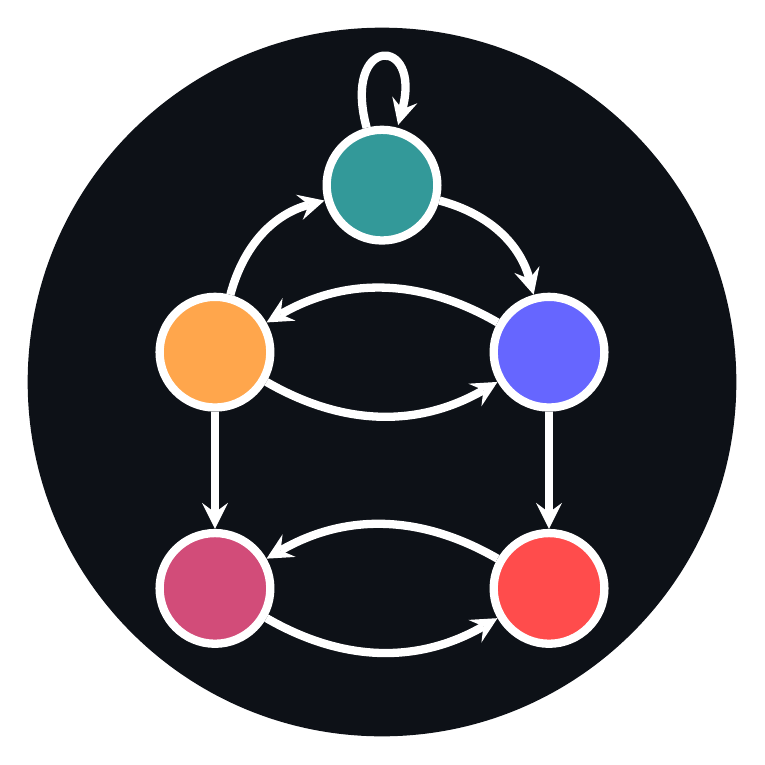
\begin{tikzpicture}[
  >=stealth, node distance=3cm, line width=3pt, white,
  element/.style={circle, draw, minimum width=4em},
]

% used in a readme to be background-free in GitHub's dark mode
\definecolor{GitHubDarkMode}{RGB}{13, 17, 23}
\fill[GitHubDarkMode] (0,-2.5) circle (4.5);

\coordinate[element, fill=teal!80] (top);
\coordinate[element, below left of=top, fill=orange!70] (mid1);
\coordinate[element, below right of=top, fill=blue!60] (mid2);
\coordinate[element, below of=mid2, fill=red!70] (bot1);
\coordinate[element, below of=mid1, fill=purple!70] (bot2);

\path[->] (top) edge[loop above] (top)
(top) edge[bend left] (mid2)
(mid1) edge[bend left] (top)
(mid2) edge[bend right] (mid1)
(mid1) edge[bend right] (mid2)
(mid1) edge (bot2)
(mid2) edge (bot1)
(bot2) edge[bend right] (bot1)
(bot1) edge[bend right] (bot2);

\end{tikzpicture}
\end{document}
